\section{Directory\-View Class Reference}
\label{classDirectoryView}\index{DirectoryView@{DirectoryView}}
{\tt \#include $<$dirview.h$>$}

\subsection*{Public Slots}
\begin{CompactItemize}
\item 
void {\bf set\-Dir} (const QString \&)
\end{CompactItemize}
\subsection*{Signals}
\begin{CompactItemize}
\item 
void {\bf folder\-Selected} (const QString \&)
\end{CompactItemize}
\subsection*{Public Member Functions}
\begin{CompactItemize}
\item 
{\bf Directory\-View} ({\bf QWidget} $\ast$parent=0, const char $\ast$name=0, bool sdo=FALSE)
\item 
bool {\bf show\-Dirs\-Only} ()
\end{CompactItemize}
\subsection*{Protected Slots}
\begin{CompactItemize}
\item 
void {\bf slot\-Folder\-Selected} (QList\-View\-Item $\ast$)
\item 
void {\bf open\-Folder} ()
\end{CompactItemize}
\subsection*{Protected Member Functions}
\begin{CompactItemize}
\item 
void {\bf contents\-Drag\-Enter\-Event} (QDrag\-Enter\-Event $\ast$e)
\item 
void {\bf contents\-Drag\-Move\-Event} (QDrag\-Move\-Event $\ast$e)
\item 
void {\bf contents\-Drag\-Leave\-Event} (QDrag\-Leave\-Event $\ast$e)
\item 
void {\bf contents\-Drop\-Event} (QDrop\-Event $\ast$e)
\item 
void {\bf contents\-Mouse\-Move\-Event} (QMouse\-Event $\ast$e)
\item 
void {\bf contents\-Mouse\-Press\-Event} (QMouse\-Event $\ast$e)
\item 
void {\bf contents\-Mouse\-Release\-Event} (QMouse\-Event $\ast$e)
\end{CompactItemize}
\subsection*{Private Member Functions}
\begin{CompactItemize}
\item 
QString {\bf full\-Path} (QList\-View\-Item $\ast$item)
\end{CompactItemize}
\subsection*{Private Attributes}
\begin{CompactItemize}
\item 
bool {\bf dirs\-Only}
\item 
QList\-View\-Item $\ast$ {\bf old\-Current}
\item 
QList\-View\-Item $\ast$ {\bf drop\-Item}
\item 
QTimer $\ast$ {\bf autoopen\_\-timer}
\item 
QPoint {\bf presspos}
\item 
bool {\bf mouse\-Pressed}
\end{CompactItemize}


\subsection{Constructor \& Destructor Documentation}
\index{DirectoryView@{Directory\-View}!DirectoryView@{DirectoryView}}
\index{DirectoryView@{DirectoryView}!DirectoryView@{Directory\-View}}
\subsubsection{\setlength{\rightskip}{0pt plus 5cm}Directory\-View::Directory\-View ({\bf QWidget} $\ast$ {\em parent} = 0, const char $\ast$ {\em name} = 0, bool {\em sdo} = FALSE)}\label{classDirectoryView_DirectoryViewa0}




Definition at line 236 of file dirview.cpp.

References autoopen\_\-timer, file\-Normal, folder\_\-locked, folder\-Closed, folder\-Locked, folder\-Open, open\-Folder(), pix\_\-file, and slot\-Folder\-Selected().



\footnotesize\begin{verbatim}237     : QListView( parent, name ), dirsOnly( sdo ), oldCurrent( 0 ),
238       dropItem( 0 ), mousePressed( FALSE )
239 {
240     autoopen_timer = new QTimer( this );
241     if ( !folderLocked ) {
242         folderLocked = new QPixmap( folder_locked );
243         folderClosed = new QPixmap( "/root/kde_application/hdass08/skin/folder_sound.png" );
244         folderOpen = new QPixmap( "/root/kde_application/hdass08/skin/folder_sound.png" );
245         fileNormal = new QPixmap( pix_file );
246     }
247 
248     connect( this, SIGNAL( doubleClicked( QListViewItem * ) ),
249              this, SLOT( slotFolderSelected( QListViewItem * ) ) );
250     connect( this, SIGNAL( returnPressed( QListViewItem * ) ),
251              this, SLOT( slotFolderSelected( QListViewItem * ) ) );
252 
253     setAcceptDrops( TRUE );
254     viewport()->setAcceptDrops( TRUE );
255 
256     connect( autoopen_timer, SIGNAL( timeout() ),
257              this, SLOT( openFolder() ) );
258 }
\end{verbatim}\normalsize 


\subsection{Member Function Documentation}
\index{DirectoryView@{Directory\-View}!contentsDragEnterEvent@{contentsDragEnterEvent}}
\index{contentsDragEnterEvent@{contentsDragEnterEvent}!DirectoryView@{Directory\-View}}
\subsubsection{\setlength{\rightskip}{0pt plus 5cm}void Directory\-View::contents\-Drag\-Enter\-Event (QDrag\-Enter\-Event $\ast$ {\em e})\hspace{0.3cm}{\tt  [protected]}}\label{classDirectoryView_DirectoryViewb0}




Definition at line 281 of file dirview.cpp.

References autoopen\_\-timer, autoopen\-Time, drop\-Item, and old\-Current.



\footnotesize\begin{verbatim}282 {
283     if ( !QUriDrag::canDecode(e) ) {
284         e->ignore();
285         return;
286     }
287 
288     oldCurrent = currentItem();
289 
290     QListViewItem *i = itemAt( contentsToViewport(e->pos()) );
291     if ( i ) {
292         dropItem = i;
293         autoopen_timer->start( autoopenTime );
294     }
295     
296 }
\end{verbatim}\normalsize 
\index{DirectoryView@{Directory\-View}!contentsDragLeaveEvent@{contentsDragLeaveEvent}}
\index{contentsDragLeaveEvent@{contentsDragLeaveEvent}!DirectoryView@{Directory\-View}}
\subsubsection{\setlength{\rightskip}{0pt plus 5cm}void Directory\-View::contents\-Drag\-Leave\-Event (QDrag\-Leave\-Event $\ast$ {\em e})\hspace{0.3cm}{\tt  [protected]}}\label{classDirectoryView_DirectoryViewb2}




Definition at line 336 of file dirview.cpp.

References autoopen\_\-timer, drop\-Item, and old\-Current.



\footnotesize\begin{verbatim}337 {
338     autoopen_timer->stop();
339     dropItem = 0;
340 
341     setCurrentItem( oldCurrent );
342     setSelected( oldCurrent, TRUE );
343 }
\end{verbatim}\normalsize 
\index{DirectoryView@{Directory\-View}!contentsDragMoveEvent@{contentsDragMoveEvent}}
\index{contentsDragMoveEvent@{contentsDragMoveEvent}!DirectoryView@{Directory\-View}}
\subsubsection{\setlength{\rightskip}{0pt plus 5cm}void Directory\-View::contents\-Drag\-Move\-Event (QDrag\-Move\-Event $\ast$ {\em e})\hspace{0.3cm}{\tt  [protected]}}\label{classDirectoryView_DirectoryViewb1}




Definition at line 299 of file dirview.cpp.

References autoopen\_\-timer, autoopen\-Time, and drop\-Item.



\footnotesize\begin{verbatim}300 {
301     if ( !QUriDrag::canDecode(e) ) {
302         e->ignore();
303         return;
304     }
305 
306     QPoint vp = contentsToViewport( ( (QDragMoveEvent*)e )->pos() );
307     QListViewItem *i = itemAt( vp );
308     
309     if ( i ) {
310         setSelected( i, TRUE );
311         e->accept();
312         if ( i != dropItem ) {
313             autoopen_timer->stop();
314             dropItem = i;
315             autoopen_timer->start( autoopenTime );
316         }
317         switch ( e->action() ) {
318         case QDropEvent::Copy:
319             break;
320         case QDropEvent::Move:
321             e->acceptAction();
322             break;
323         case QDropEvent::Link:
324             e->acceptAction();
325             break;
326         default:
327             ;
328         }
329     } else {
330         e->ignore();
331         autoopen_timer->stop();
332         dropItem = 0;
333     }
334 }
\end{verbatim}\normalsize 
\index{DirectoryView@{Directory\-View}!contentsDropEvent@{contentsDropEvent}}
\index{contentsDropEvent@{contentsDropEvent}!DirectoryView@{Directory\-View}}
\subsubsection{\setlength{\rightskip}{0pt plus 5cm}void Directory\-View::contents\-Drop\-Event (QDrop\-Event $\ast$ {\em e})\hspace{0.3cm}{\tt  [protected]}}\label{classDirectoryView_DirectoryViewb3}




Definition at line 345 of file dirview.cpp.

References autoopen\_\-timer, and full\-Path().



\footnotesize\begin{verbatim}346 {
347     autoopen_timer->stop();
348 
349     if ( !QUriDrag::canDecode(e) ) {
350         e->ignore();
351         return;
352     }
353 
354     QListViewItem *item = itemAt( contentsToViewport(e->pos()) );
355     
356     if(item)
357     {
358         //DAVID make a list to receive the dropping objects
359         QStrList lst;
360         
361         //DAVID decode the objects data to list
362         QUriDrag::decode( e, lst );
363         
364         QString DirName=QDir::convertSeparators(fullPath(item));
365 
366         for ( uint i = 0; i < lst.count(); ++i ) 
367         
368         {
369                 
370                 //kdDebug()<<lst.at(i);
371                 //DAVID get the dropping object name
372                 QString fullpathfilename = QDir::convertSeparators(QUriDrag::uriToLocalFile(lst.at(i)));
373                 QUrl url(fullpathfilename);
374                 QString filename=url.fileName();
375                 QString distfilename=DirName+QString("/")+filename;
376                 //copy file
377                 KIO::copy(KURL(fullpathfilename),KURL(distfilename),false);
378         }
379         
380     }
381     else
382     {
383      e->ignore();
384     }
385 
386 }
\end{verbatim}\normalsize 


Here is the call graph for this function:\begin{figure}[H]
\begin{center}
\leavevmode
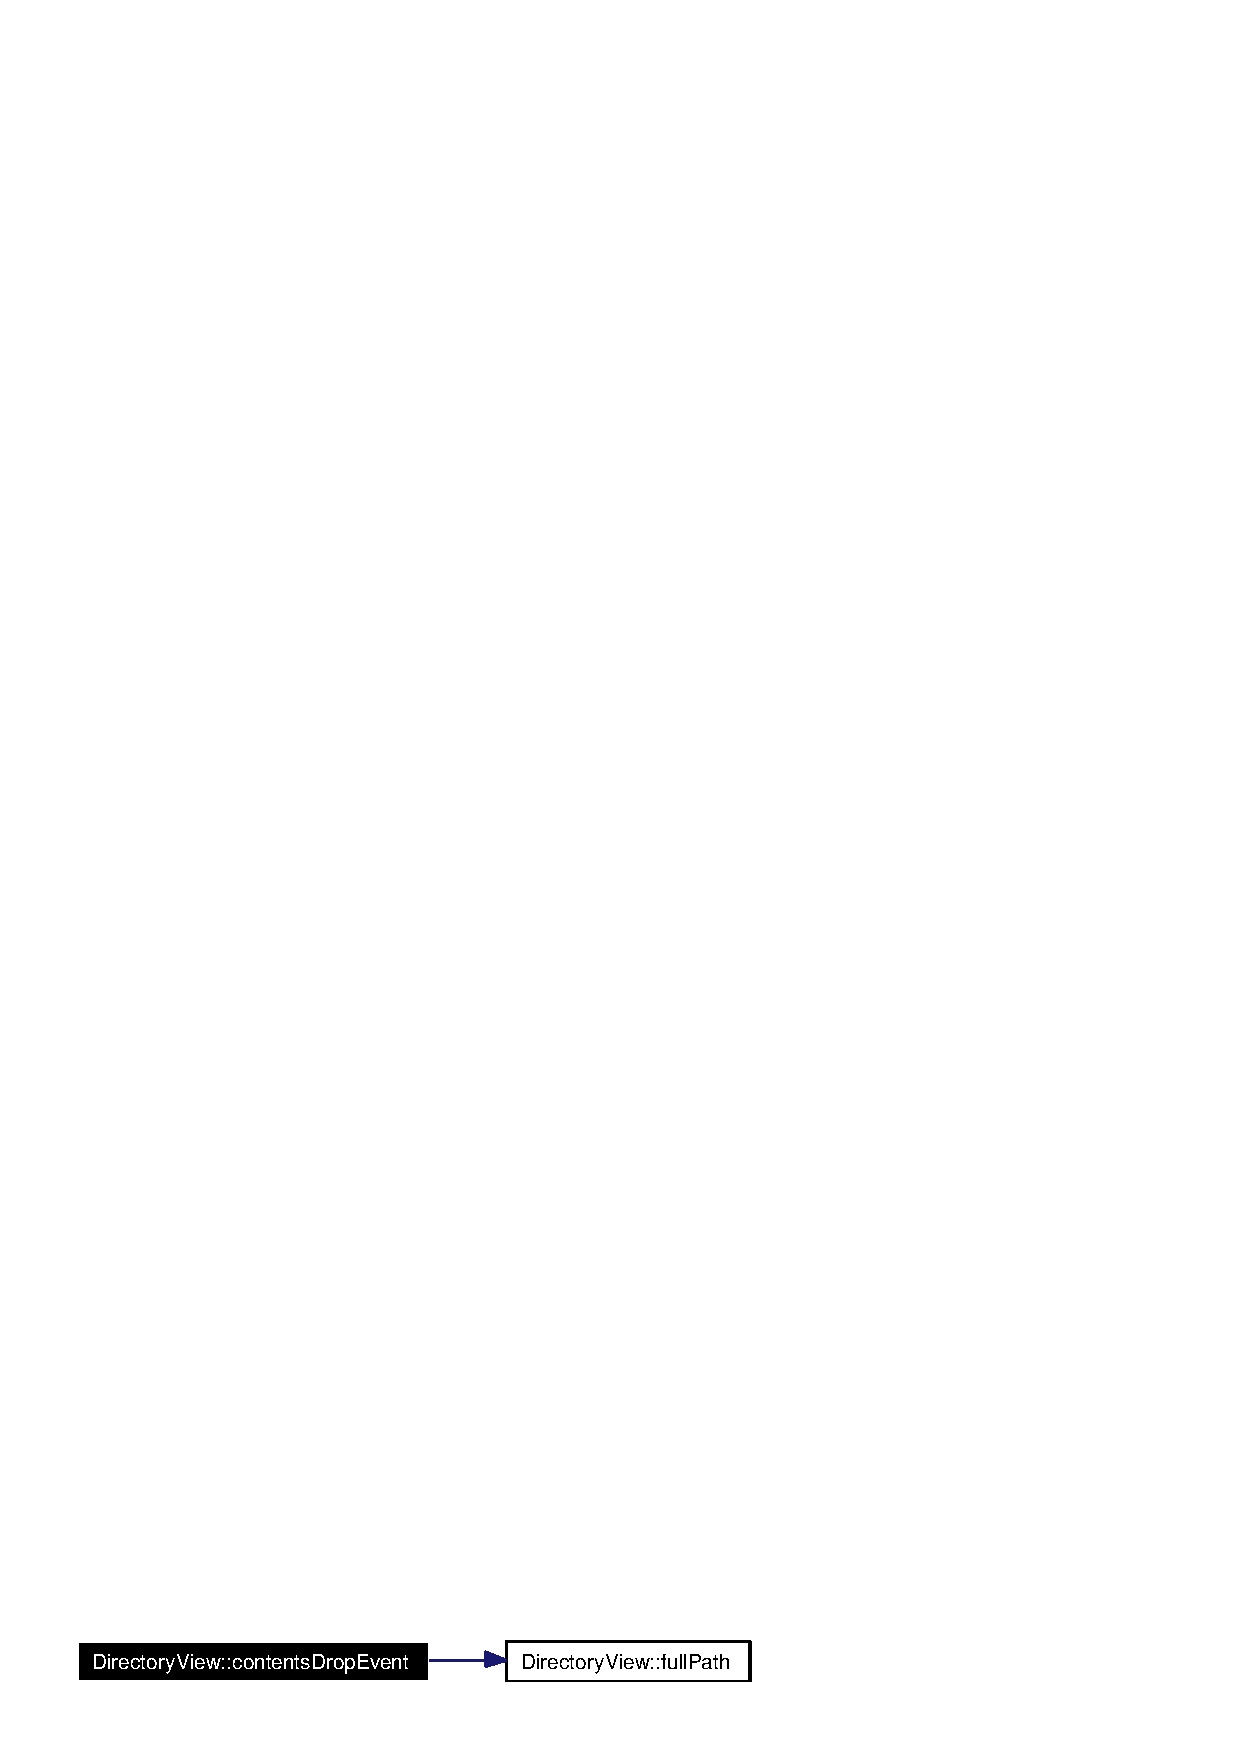
\includegraphics[width=180pt]{classDirectoryView_DirectoryViewb3_cgraph}
\end{center}
\end{figure}
\index{DirectoryView@{Directory\-View}!contentsMouseMoveEvent@{contentsMouseMoveEvent}}
\index{contentsMouseMoveEvent@{contentsMouseMoveEvent}!DirectoryView@{Directory\-View}}
\subsubsection{\setlength{\rightskip}{0pt plus 5cm}void Directory\-View::contents\-Mouse\-Move\-Event (QMouse\-Event $\ast$ {\em e})\hspace{0.3cm}{\tt  [protected]}}\label{classDirectoryView_DirectoryViewb4}




Definition at line 424 of file dirview.cpp.

References full\-Path(), mouse\-Pressed, and presspos.



\footnotesize\begin{verbatim}425 {
426     if ( mousePressed && ( presspos - e->pos() ).manhattanLength() > QApplication::startDragDistance() ) {
427         mousePressed = FALSE;
428         QListViewItem *item = itemAt( contentsToViewport(presspos) );
429         if ( item ) {
430             QString source = fullPath(item);
431             if ( QFile::exists(source) ) {
432                 QUriDrag* ud = new QUriDrag(viewport());
433                 ud->setFileNames( source );
434                 if ( ud->drag() )
435                     QMessageBox::information( this, "Drag source",
436                     QString("Delete ") + QDir::convertSeparators(source), "Not implemented" );
437             }
438         }
439     }
440 }
\end{verbatim}\normalsize 


Here is the call graph for this function:\begin{figure}[H]
\begin{center}
\leavevmode
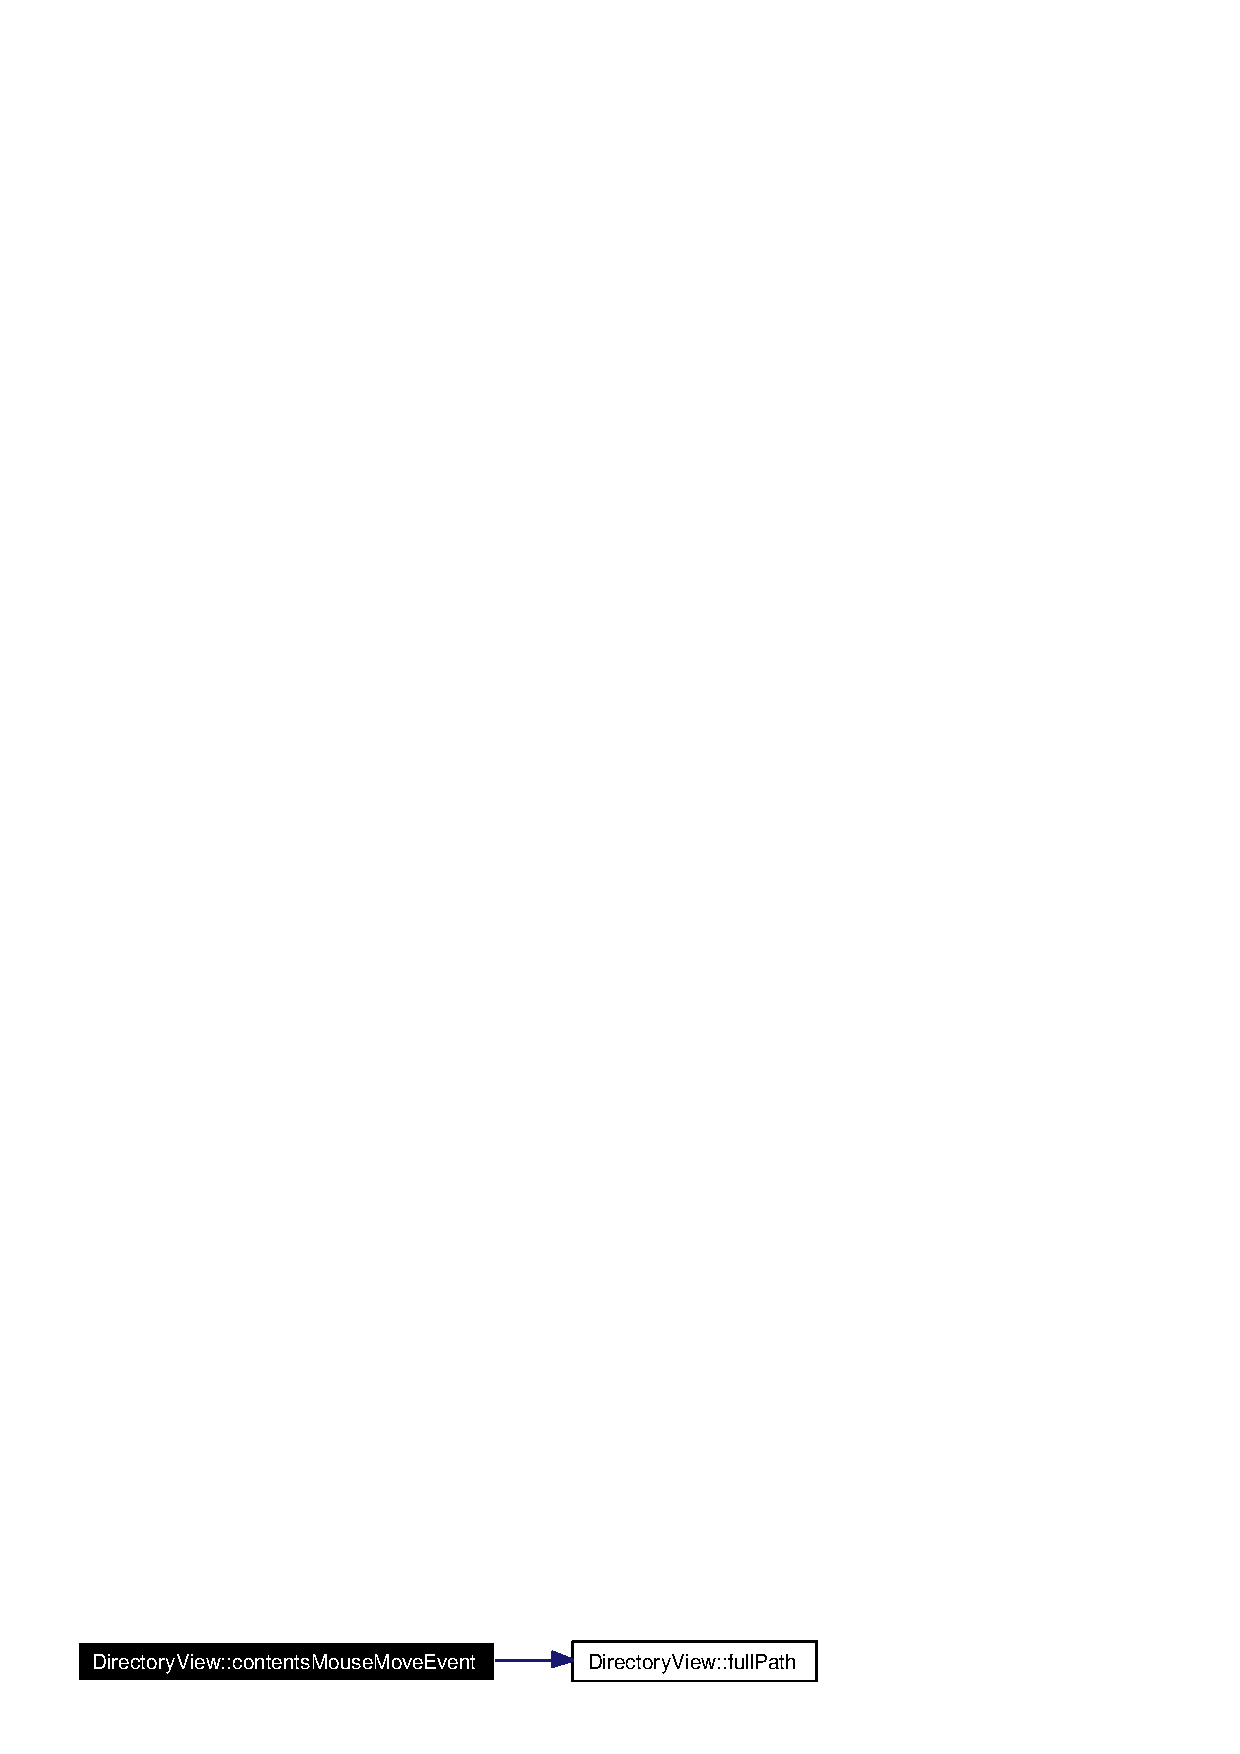
\includegraphics[width=196pt]{classDirectoryView_DirectoryViewb4_cgraph}
\end{center}
\end{figure}
\index{DirectoryView@{Directory\-View}!contentsMousePressEvent@{contentsMousePressEvent}}
\index{contentsMousePressEvent@{contentsMousePressEvent}!DirectoryView@{Directory\-View}}
\subsubsection{\setlength{\rightskip}{0pt plus 5cm}void Directory\-View::contents\-Mouse\-Press\-Event (QMouse\-Event $\ast$ {\em e})\hspace{0.3cm}{\tt  [protected]}}\label{classDirectoryView_DirectoryViewb5}




Definition at line 408 of file dirview.cpp.

References mouse\-Pressed, and presspos.



\footnotesize\begin{verbatim}409 {
410     QListView::contentsMousePressEvent(e);
411     QPoint p( contentsToViewport( e->pos() ) );
412     QListViewItem *i = itemAt( p );
413     if ( i ) {
414         // if the user clicked into the root decoration of the item, don't try to start a drag!
415         if ( p.x() > header()->cellPos( header()->mapToActual( 0 ) ) +
416              treeStepSize() * ( i->depth() + ( rootIsDecorated() ? 1 : 0) ) + itemMargin() ||
417              p.x() < header()->cellPos( header()->mapToActual( 0 ) ) ) {
418             presspos = e->pos();
419             mousePressed = TRUE;
420         }
421     }
422 }
\end{verbatim}\normalsize 
\index{DirectoryView@{Directory\-View}!contentsMouseReleaseEvent@{contentsMouseReleaseEvent}}
\index{contentsMouseReleaseEvent@{contentsMouseReleaseEvent}!DirectoryView@{Directory\-View}}
\subsubsection{\setlength{\rightskip}{0pt plus 5cm}void Directory\-View::contents\-Mouse\-Release\-Event (QMouse\-Event $\ast$ {\em e})\hspace{0.3cm}{\tt  [protected]}}\label{classDirectoryView_DirectoryViewb6}




Definition at line 442 of file dirview.cpp.

References mouse\-Pressed.



\footnotesize\begin{verbatim}443 {
444     mousePressed = FALSE;
445 }
\end{verbatim}\normalsize 
\index{DirectoryView@{Directory\-View}!folderSelected@{folderSelected}}
\index{folderSelected@{folderSelected}!DirectoryView@{Directory\-View}}
\subsubsection{\setlength{\rightskip}{0pt plus 5cm}void Directory\-View::folder\-Selected (const QString \&)\hspace{0.3cm}{\tt  [signal]}}\label{classDirectoryView_DirectoryViewl0}




Definition at line 97 of file dirview.moc.cc.

Referenced by slot\-Folder\-Selected().



\footnotesize\begin{verbatim}98 {
99     activate_signal( staticMetaObject()->signalOffset() + 0, t0 );
100 }
\end{verbatim}\normalsize 
\index{DirectoryView@{Directory\-View}!fullPath@{fullPath}}
\index{fullPath@{fullPath}!DirectoryView@{Directory\-View}}
\subsubsection{\setlength{\rightskip}{0pt plus 5cm}QString Directory\-View::full\-Path (QList\-View\-Item $\ast$ {\em item})\hspace{0.3cm}{\tt  [private]}}\label{classDirectoryView_DirectoryViewd0}




Definition at line 389 of file dirview.cpp.

Referenced by contents\-Drop\-Event(), and contents\-Mouse\-Move\-Event().



\footnotesize\begin{verbatim}390 {
391     QString fullpath = item->text(0);
392     while ( (item=item->parent()) ) {
393         if ( item->parent() )
394             fullpath = item->text(0) + "/" + fullpath;
395         else
396             fullpath = item->text(0) + fullpath;
397     }
398 #ifdef Q_WS_WIN
399         if (fullpath.length() > 2 && fullpath[1] != ':') {
400                 QDir dir(fullpath);
401                 fullpath = dir.currentDirPath().left(2) + fullpath;
402         }
403 #endif
404         
405     return fullpath;
406 }
\end{verbatim}\normalsize 
\index{DirectoryView@{Directory\-View}!openFolder@{openFolder}}
\index{openFolder@{openFolder}!DirectoryView@{Directory\-View}}
\subsubsection{\setlength{\rightskip}{0pt plus 5cm}void Directory\-View::open\-Folder ()\hspace{0.3cm}{\tt  [protected, slot]}}\label{classDirectoryView_DirectoryViewj1}




Definition at line 269 of file dirview.cpp.

References autoopen\_\-timer, and drop\-Item.

Referenced by Directory\-View().



\footnotesize\begin{verbatim}270 {
271     autoopen_timer->stop();
272     if ( dropItem && !dropItem->isOpen() ) {
273         dropItem->setOpen( TRUE );
274         dropItem->repaint();
275     }
276 }
\end{verbatim}\normalsize 
\index{DirectoryView@{Directory\-View}!setDir@{setDir}}
\index{setDir@{setDir}!DirectoryView@{Directory\-View}}
\subsubsection{\setlength{\rightskip}{0pt plus 5cm}void Directory\-View::set\-Dir (const QString \&)\hspace{0.3cm}{\tt  [slot]}}\label{classDirectoryView_DirectoryViewi0}




Definition at line 447 of file dirview.cpp.



\footnotesize\begin{verbatim}448 {
449     QListViewItemIterator it( this );
450     ++it;
451     for ( ; it.current(); ++it ) {
452         it.current()->setOpen( FALSE );
453     }
454 
455     QStringList lst( QStringList::split( "/", s ) );
456     QListViewItem *item = firstChild();
457     QStringList::Iterator it2 = lst.begin();
458     for ( ; it2 != lst.end(); ++it2 ) {
459         while ( item ) {
460             if ( item->text( 0 ) == *it2 ) {
461                 item->setOpen( TRUE );
462                 break;
463             }
464             item = item->itemBelow();
465         }
466     }
467 
468     if ( item )
469         setCurrentItem( item );
470 }
\end{verbatim}\normalsize 
\index{DirectoryView@{Directory\-View}!showDirsOnly@{showDirsOnly}}
\index{showDirsOnly@{showDirsOnly}!DirectoryView@{Directory\-View}}
\subsubsection{\setlength{\rightskip}{0pt plus 5cm}bool Directory\-View::show\-Dirs\-Only ()\hspace{0.3cm}{\tt  [inline]}}\label{classDirectoryView_DirectoryViewa1}




Definition at line 80 of file dirview.h.

References dirs\-Only.

Referenced by slot\-Folder\-Selected().



\footnotesize\begin{verbatim}80 { return dirsOnly; }
\end{verbatim}\normalsize 
\index{DirectoryView@{Directory\-View}!slotFolderSelected@{slotFolderSelected}}
\index{slotFolderSelected@{slotFolderSelected}!DirectoryView@{Directory\-View}}
\subsubsection{\setlength{\rightskip}{0pt plus 5cm}void Directory\-View::slot\-Folder\-Selected (QList\-View\-Item $\ast$)\hspace{0.3cm}{\tt  [protected, slot]}}\label{classDirectoryView_DirectoryViewj0}




Definition at line 260 of file dirview.cpp.

References folder\-Selected(), Directory::full\-Name(), and show\-Dirs\-Only().

Referenced by Directory\-View().



\footnotesize\begin{verbatim}261 {
262     if ( !i || !showDirsOnly() )
263         return;
264 
265     Directory *dir = (Directory*)i;
266     emit folderSelected( dir->fullName() );
267 }
\end{verbatim}\normalsize 


\subsection{Member Data Documentation}
\index{DirectoryView@{Directory\-View}!autoopen_timer@{autoopen\_\-timer}}
\index{autoopen_timer@{autoopen\_\-timer}!DirectoryView@{Directory\-View}}
\subsubsection{\setlength{\rightskip}{0pt plus 5cm}QTimer$\ast$ {\bf Directory\-View::autoopen\_\-timer}\hspace{0.3cm}{\tt  [private]}}\label{classDirectoryView_DirectoryViewr3}




Definition at line 106 of file dirview.h.

Referenced by contents\-Drag\-Enter\-Event(), contents\-Drag\-Leave\-Event(), contents\-Drag\-Move\-Event(), contents\-Drop\-Event(), Directory\-View(), and open\-Folder().\index{DirectoryView@{Directory\-View}!dirsOnly@{dirsOnly}}
\index{dirsOnly@{dirsOnly}!DirectoryView@{Directory\-View}}
\subsubsection{\setlength{\rightskip}{0pt plus 5cm}bool {\bf Directory\-View::dirs\-Only}\hspace{0.3cm}{\tt  [private]}}\label{classDirectoryView_DirectoryViewr0}




Definition at line 103 of file dirview.h.

Referenced by show\-Dirs\-Only().\index{DirectoryView@{Directory\-View}!dropItem@{dropItem}}
\index{dropItem@{dropItem}!DirectoryView@{Directory\-View}}
\subsubsection{\setlength{\rightskip}{0pt plus 5cm}QList\-View\-Item$\ast$ {\bf Directory\-View::drop\-Item}\hspace{0.3cm}{\tt  [private]}}\label{classDirectoryView_DirectoryViewr2}




Definition at line 105 of file dirview.h.

Referenced by contents\-Drag\-Enter\-Event(), contents\-Drag\-Leave\-Event(), contents\-Drag\-Move\-Event(), and open\-Folder().\index{DirectoryView@{Directory\-View}!mousePressed@{mousePressed}}
\index{mousePressed@{mousePressed}!DirectoryView@{Directory\-View}}
\subsubsection{\setlength{\rightskip}{0pt plus 5cm}bool {\bf Directory\-View::mouse\-Pressed}\hspace{0.3cm}{\tt  [private]}}\label{classDirectoryView_DirectoryViewr5}




Definition at line 108 of file dirview.h.

Referenced by contents\-Mouse\-Move\-Event(), contents\-Mouse\-Press\-Event(), and contents\-Mouse\-Release\-Event().\index{DirectoryView@{Directory\-View}!oldCurrent@{oldCurrent}}
\index{oldCurrent@{oldCurrent}!DirectoryView@{Directory\-View}}
\subsubsection{\setlength{\rightskip}{0pt plus 5cm}QList\-View\-Item$\ast$ {\bf Directory\-View::old\-Current}\hspace{0.3cm}{\tt  [private]}}\label{classDirectoryView_DirectoryViewr1}




Definition at line 104 of file dirview.h.

Referenced by contents\-Drag\-Enter\-Event(), and contents\-Drag\-Leave\-Event().\index{DirectoryView@{Directory\-View}!presspos@{presspos}}
\index{presspos@{presspos}!DirectoryView@{Directory\-View}}
\subsubsection{\setlength{\rightskip}{0pt plus 5cm}QPoint {\bf Directory\-View::presspos}\hspace{0.3cm}{\tt  [private]}}\label{classDirectoryView_DirectoryViewr4}




Definition at line 107 of file dirview.h.

Referenced by contents\-Mouse\-Move\-Event(), and contents\-Mouse\-Press\-Event().

The documentation for this class was generated from the following files:\begin{CompactItemize}
\item 
{\bf dirview.h}\item 
{\bf dirview.moc.cc}\item 
{\bf dirview.cpp}\end{CompactItemize}
